\documentclass[a4paper, 11pt, lualatex, ja=standard]{bxjsarticle}

\usepackage{graphicx} % 画像
\usepackage{tabularx} % 表

\usepackage{amsmath}  % 数式
\usepackage{empheq}   % 連立方程式
\usepackage{url}      % URL
\usepackage{siunitx}  % SI単位

% フォント設定
\usepackage[no-math, deluxe, bold, haranoaji]{luatexja-preset}

\usepackage{layout}   % レイアウト確認

\renewcommand{\tablename}{Table}    % 表番号フォーマットをTableへ
\renewcommand{\figurename}{Fig.}    % 図番号フォーマットをFig.へ

\renewcommand{\baselinestretch}{0.8}    % 行間の調整

\title{\huge 4輪メカナムホイールの逆運動学}
\author{\large fjnkt98}
\date{\today}

\begin{document}
  \maketitle
  
  \section{目的}

4輪メカナムホイールロボットの制御を行うために逆運動学を求める.
  \section{逆運動学及び順運動学の導出}

ここでは図\ref{fig:mecanum}に示すメカナムホイールロボットの運動学を導出する.

\begin{figure}[h]
  \centering
  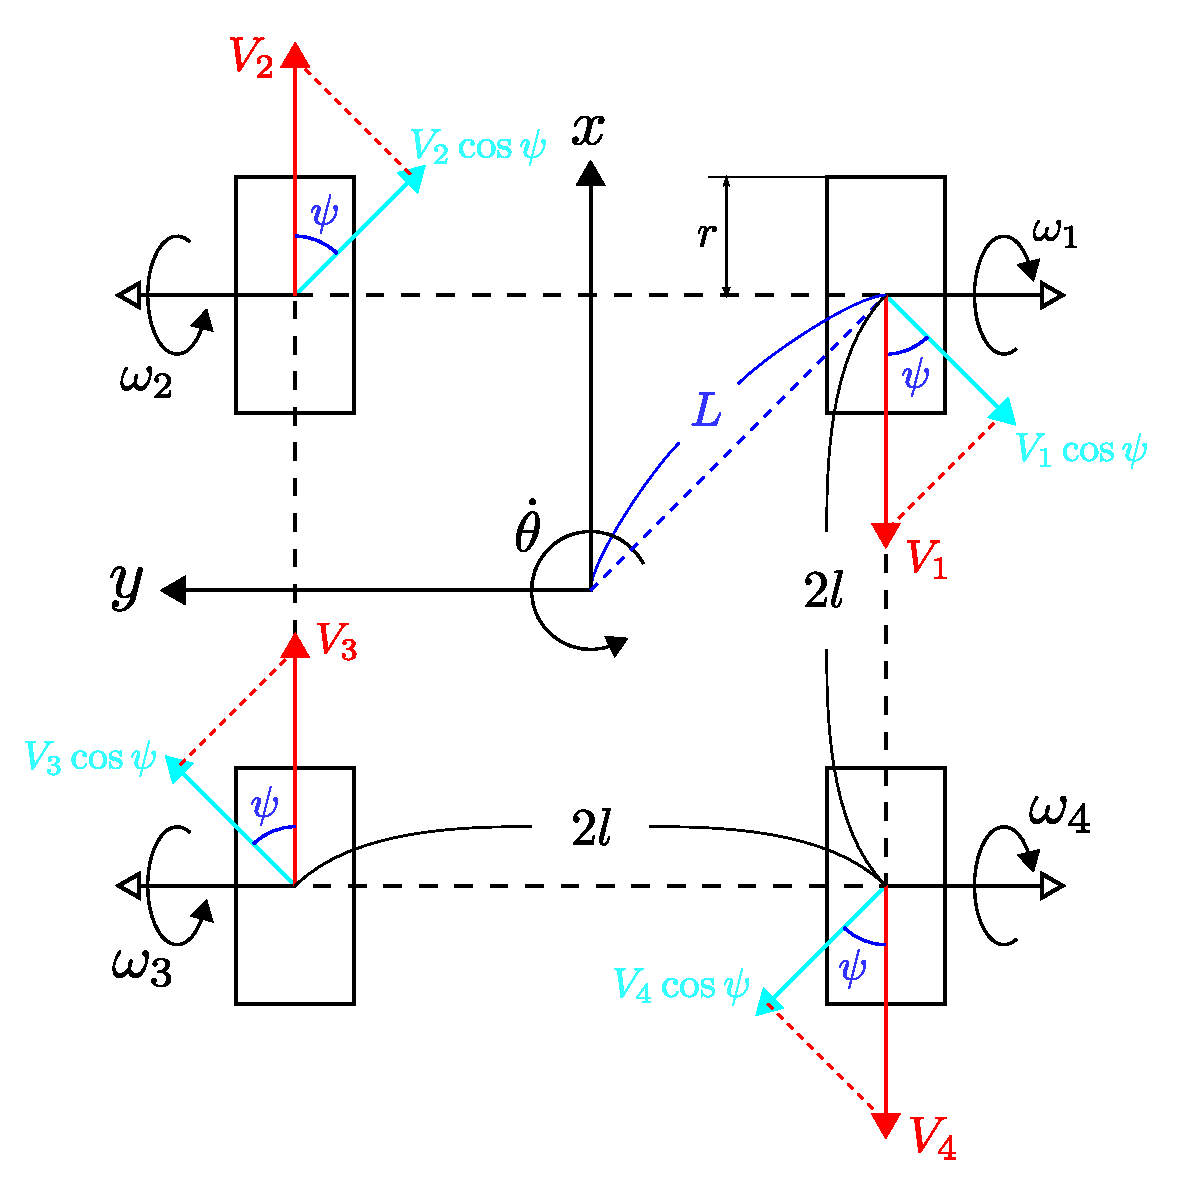
\includegraphics[width=120truemm, clip]{images/mecanum.pdf}
  \caption{4WD Mecanum Wheel}
  \label{fig:mecanum}
\end{figure}

\subsection{ロボットの各種パラメータ}

ロボット座標系は右手系座標系であり,原点はロボットの中心に固定されている.
$x$軸はロボットの前進方向に,$z$軸は鉛直上方向に設定されている.



ロボットは次のパラメータを持つ.

\begin{itemize}
  \item メカナムホイールの半径$r$
  \item ホイールのローラ角度$\psi =$\ang{45}
  \item ホイール間距離$2l$
  \item ロボット中心からホイールまでの距離$L = \sqrt{2}l$
  \item ホイール角速度$\omega_{i}$
  \item ホイールの周速度$V_{i} = r\omega_{i}$
  \item ロボットの速度の$x$軸方向成分$\dot{x}$
  \item ロボットの速度の$y$軸方向成分$\dot{y}$
  \item ロボットの角速度$\dot{\theta}$
\end{itemize}

メカナムホイールロボットはホイールが正方形の頂点上に配置されているタイプのものを考える.
また,ホイールのローラ角度は\ang{45}とする.

\subsection{逆運動学の導出}

メカナムホイールが回転すると,接地しているローラの軸方向に速度を発生させる.
その大きさはメカナムホイールの周速度$V_{i}$に$\cos{\psi}$を乗じたものになる.
ロボットの速度はホイールによってのみ発生することを考えると,式\ref{eq:inv1}が成り立つ.

\begin{subequations}
  \begin{empheq}[left=\empheqlbrace]{align}
    V_{1}\cos{\psi} &= - \dot{x}\cos{\psi} - \dot{y}\sin{\psi} - L\dot{\theta} \\
    V_{2}\cos{\psi} &=   \dot{x}\cos{\psi} - \dot{y}\sin{\psi} - L\dot{\theta} \\
    V_{3}\cos{\psi} &=   \dot{x}\cos{\psi} + \dot{y}\sin{\psi} - L\dot{\theta} \\
    V_{4}\cos{\psi} &= - \dot{x}\cos{\psi} + \dot{y}\sin{\psi} - L\dot{\theta}
  \end{empheq}
  \label{eq:inv1}
\end{subequations}

式\ref{eq:inv1}に$\psi =$\ang{45}を代入すると,式\ref{eq:inv2}が得られる.

\begin{subequations}
  \begin{empheq}[left=\empheqlbrace]{align}
    \frac{\sqrt{2}}{2} V_{1} &= - \frac{\sqrt{2}}{2}\dot{x} - \frac{\sqrt{2}}{2}\dot{y} - L\dot{\theta} \\
    \frac{\sqrt{2}}{2} V_{2} &= \frac{\sqrt{2}}{2}\dot{x} - \frac{\sqrt{2}}{2}\dot{y} - L\dot{\theta} \\
    \frac{\sqrt{2}}{2} V_{3} &= \frac{\sqrt{2}}{2}\dot{x} + \frac{\sqrt{2}}{2}\dot{y} - L\dot{\theta} \\
    \frac{\sqrt{2}}{2} V_{4} &= - \frac{\sqrt{2}}{2}\dot{x} + \frac{\sqrt{2}}{2}\dot{y} - L\dot{\theta}
  \end{empheq}
  \label{eq:inv2}
\end{subequations}

$\sqrt{2} L = \sqrt{2} \times \sqrt{l^2 + l^2} = 2l$であることを考慮して式\ref{eq:inv2}を変形すると,式\ref{eq:inv3}が得られる.

\begin{subequations}
  \begin{empheq}[left=\empheqlbrace]{align}
    V_{1} &= - \dot{x} - \dot{y} - 2l\dot{\theta} \\
    V_{2} &= \dot{x} - \dot{y} - 2l\dot{\theta} \\
    V_{3} &= \dot{x} + \dot{y} - 2l\dot{\theta} \\
    V_{4} &= - \dot{x} +\dot{y} - 2l\dot{\theta}
  \end{empheq}
  \label{eq:inv3}
\end{subequations}

式\ref{eq:inv3}を行列表示すると式\ref{eq:inv4}が得られる.

\begin{equation}
  \begin{pmatrix}
    V_{1} \\ V_{2} \\ V_{3} \\ V_{4}
  \end{pmatrix}
  =
  \begin{pmatrix}
     -1 & -1 & -2l \\
     1 & -1 & -2l \\
     1 & 1 & -2l \\
     -1 & 1 & -2l
  \end{pmatrix}
  \begin{pmatrix}
    \dot{x} \\
    \dot{y} \\
    \dot{\theta}
  \end{pmatrix}
  \label{eq:inv4}
\end{equation}

\subsection{順運動学の導出}

順運動学は,逆運動学の式を変形することで得られる.
今,式\ref{eq:inv4}の係数行列を$A$と置く.

\begin{equation*}
  \begin{pmatrix}
    V_{1} \\ V_{2} \\ V_{3} \\ V_{4}
  \end{pmatrix}
  =
  A
  \begin{pmatrix}
    \dot{x} \\
    \dot{y} \\
    \dot{\theta}
  \end{pmatrix}
  \label{eq:inv4}
\end{equation*}

順運動学を求めるには,$A$の逆行列$A^{-1}$を求めればよい.
しかし,$A$は正方行列ではないため,逆行列を持たない.
従って,疑似逆行列を用いる.
$A$の疑似逆行列$A^{+}$は$A^{+} = (A^{T}A)^{-1}A^{T}$で求められる.
これにより$A^{+}$が次のように求まる.

\begin{equation}
  A^{+} = \frac{1}{4}
  \begin{pmatrix}
    -1 & 1 & 1 & -1 \\
    -1 & -1 & 1 & 1 \\
    -\frac{1}{2l} & -\frac{1}{2l} & -\frac{1}{2l} & -\frac{1}{2l}
  \end{pmatrix}
\end{equation}

従って,式\ref{eq:forward}に示す順運動学が求まる.

\begin{equation}
  \begin{pmatrix}
    \dot{x} \\
    \dot{y} \\
    \dot{\theta}
  \end{pmatrix}
  =
  \begin{pmatrix}
    -1 & 1 & 1 & -1 \\
    -1 & -1 & 1 & 1 \\
    -\frac{1}{2l} & -\frac{1}{2l} & -\frac{1}{2l} & -\frac{1}{2l}
  \end{pmatrix}
  \begin{pmatrix}
    V_{1} \\ V_{2} \\ V_{3} \\ V_{4}
  \end{pmatrix}
  \label{eq:forward}
\end{equation}
  \section{速度制御のための入力変換}

前章では4輪メカナムホイールロボットの逆運動学及び順運動学を導いた.
ロボットを操縦する際は,速度ベクトル$\vec{x} = (\dot{x}, \dot{y}, \dot{\theta})^T$を入力として,逆運動学により各ホイールの速度を計算するのが一般的だが,入力できる速度には制限がある.
メカナムホイールのような全方位移動ロボットのコントローラとしては3軸のジョイスティックが用いられるのが一般的であるが,それぞれのジョイスティックをそのまま各速度に対応させるのは適切ではない.
そこで,コントローラからの3軸入力を,ロボットへの入力速度ベクトルへとマッピングする処理が必要となる.

\subsection{入力速度の制約式}

ロボットの移動速度はホイールの最大回転速度により制限される.式\ref{eq:inv3}を見ると分かるように,ロボットへの入力速度$\dot{x}$,$\dot{y}$,$\dot{\theta}$は,その絶対値の和がホイールの出せる最大回転速度を超えるような組み合わせになってはならない.
ここで,各ホイールの性能は全て同等とし,ホイールが出せる最大角速度を$\omega_{\text{max}}$,ホイールの最大周速度を$V_{\text{max}} = r \omega_{\text{max}}$とすると,式\ref{eq:constraint}に示す入力速度の制約式が得られる.

\begin{equation}
  V_{\text{max}} = |\dot{x}| + |\dot{y}| + 2l|\dot{\theta}|
  \label{eq:constraint}
\end{equation}

ここで,$\hat{\dot{\theta}} = 2l\dot{\theta}$として式\ref{eq:constraint}に代入すると,式\ref{eq:constraint}は図に示すような$\dot{x}\dot{y}\hat{\dot{\theta}}$座標系における正八面体の内部領域を表す.
ロボットへの入力速度ベクトル$\vec{x} = (\dot{x}, \dot{y}, \dot{\theta})^T$をこの座標系の位置ベクトルであるとしたとき,位置ベクトルは正八面体の内部に存在していなければならない.

\begin{figure}[h]
  \centering
  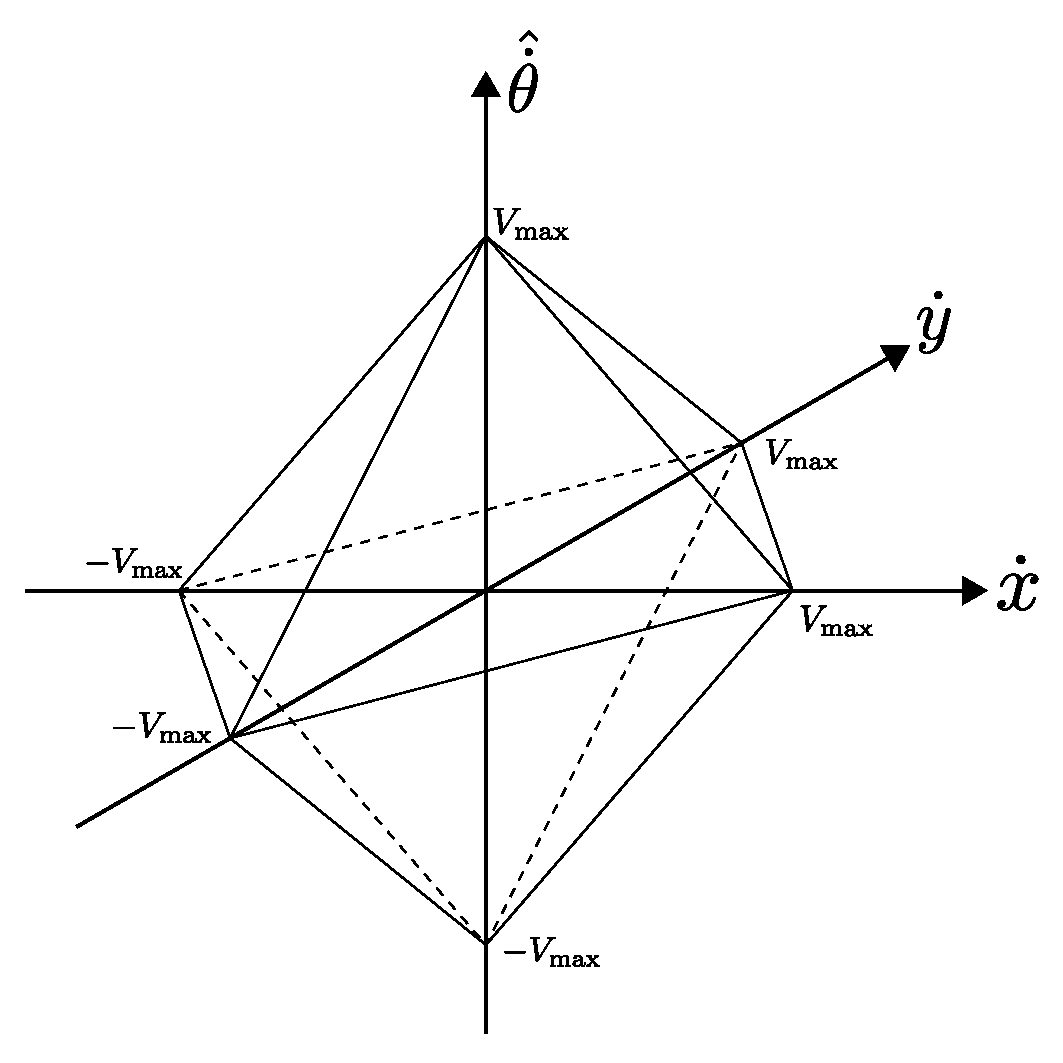
\includegraphics[width=80truemm, clip]{images/constraint.pdf}
  \caption{Constraint Area of Input Velocity Vector}
  \label{fig:constraint}
\end{figure}

\subsection{入力信号から速度ベクトルへのマッピング}

\subsubsection{コントローラからの入力信号}

ここでは3軸のアナログジョイスティックを用いてロボットを速度制御することを考える.
それぞれのアナログジョイスティックの入力は$\dot{x}$,$\dot{y}$,$\hat{\dot{\theta}}$に対応するものとし,$\dot{x}$に対応するアナログジョイスティックの信号値を$\alpha$,$\dot{y}$に対応するものを$\beta$,$\hat{\dot{\theta}}$に対応するものを$\gamma$と表す.
また,各ジョイスティックの信号値の範囲は-1.0~1.0であるとする.

3つのジョイスティックによる入力の組み合わせをベクトル$\vec{\epsilon} = (\alpha, \beta, \gamma)^T$で表す.
$\alpha\beta\gamma$座標系において,$\vec{\epsilon}$が取る領域は,原点を中心とする幅2の正方形となる.
この正方形の領域を,図\ref{fig:constraint}に示す正八面体にマッピングすることで,ジョイスティックによる制御が可能になる.

\begin{figure}[h]
  \centering
  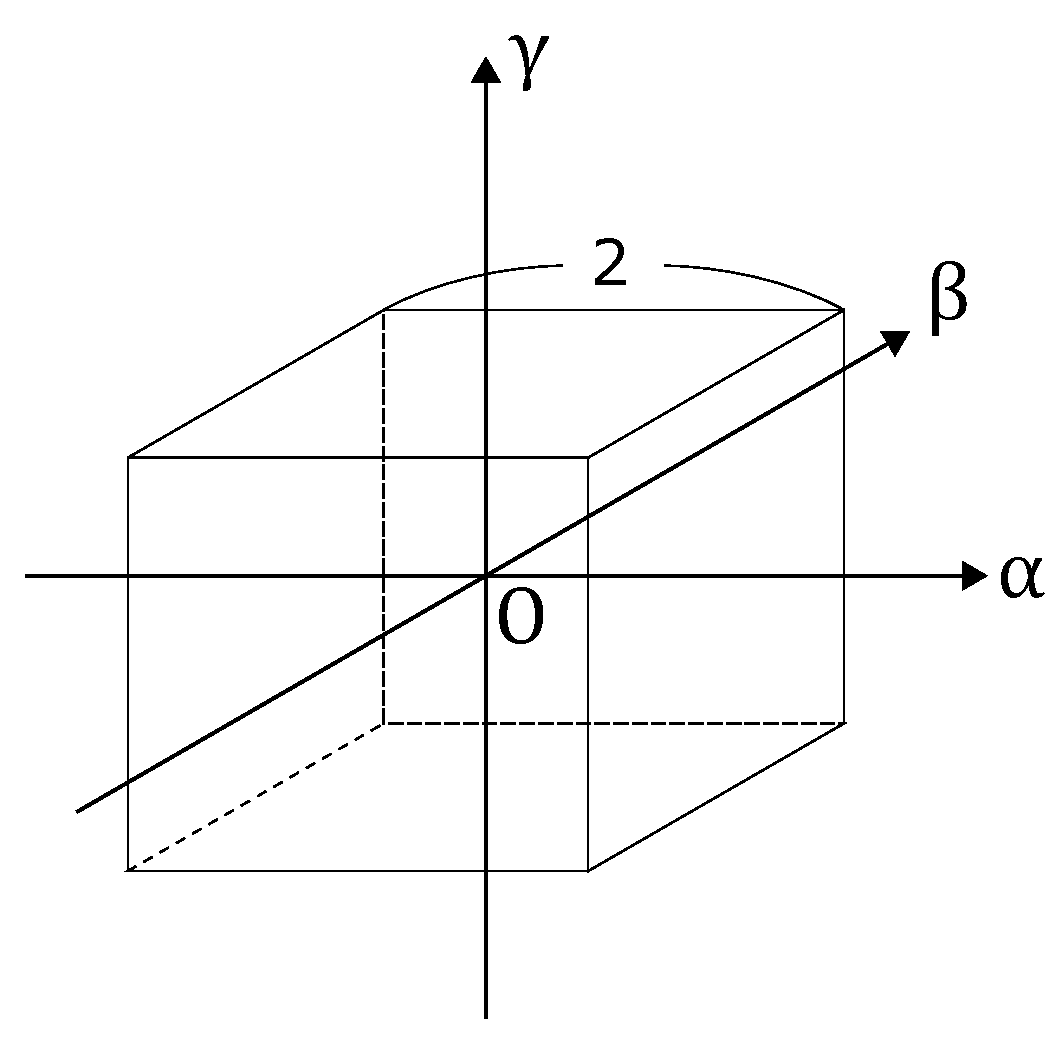
\includegraphics[width=80truemm, clip]{images/input.pdf}
  \caption{Input Area}
  \label{fig:input}
\end{figure}

\subsubsection{極座標変換によるアプローチ}

正方形領域から正八面体領域へのマッピングを直接行うのは困難であるため,ここでは極座標変換を用いたマッピング処理を行う.

まず,$\alpha\beta\gamma$座標系における正方形領域を3次元極座標における球面へ変換する.
入力信号ベクトル$\vec{\epsilon}$の向きと大きさを求める.
\end{document}